%! Author = Philipp Emmenegger
%! Date = 30/06/2021
\subsection*{Abkürzungen}
\begin{itemize}
    \item \textbf{ADAM} Adaptive Moment Estimation
    \item \textbf{ANN} Artificial Neural Network
    \item \textbf{KNN} K Nearest Neighbour
    \item \textbf{MSE} Mean Squared Error
    \item \textbf{MLE} Maximum Likelihood Estimation
    \item \textbf{NLP} Natural Language Processing
    \item \textbf{OLS} Ordinary Least Squares
    \item \textbf{PMF} Probability Mass Function (Wahrscheinlichkeitsfunktion)
    \item \textbf{ROC} Receiver Operating Characteristics
    \item \textbf{SGD} Stochastic Gradient Descent 
    \item \textbf{WCSS} within-cluster sum-of-squares
\end{itemize}

\section{Introduction}
\textbf{Artificial Intelligence}
\begin{itemize}
    \item broad concept
    \item different interpretations
    \item we do not have a definition of inteligence
\end{itemize}
\textbf{Statistical machine learning}
\begin{itemize}
    \item Algorithms and applications where computer learn from data
\end{itemize}
\textbf{AGI}
\begin{itemize}
    \item Artificial General Intelligence
    \item Hypothetical computer program that can perform intellectual tasks as well as, or better than a human.
\end{itemize}
\textbf{Turing Test}
\begin{itemize}
    \item Also called imitation game
    \item Tests of a machine's ability to exhibit intelligent behaviour equivalent to, or indistinguishable from that of a human
    \item Has some philosophical problems (Complex problems, humans cant solve / AI must learn to lie)
\end{itemize}
\textbf{Examples of application (today):}
\begin{itemize}
    \item Personalization of news feeds
    \item Product searching and recommendation s on eCommerce platforms
    \item Voice-to-text
    \item Predictive maintenance
\end{itemize}
\subsection{Tasks and Algorithms of Machine Learning}
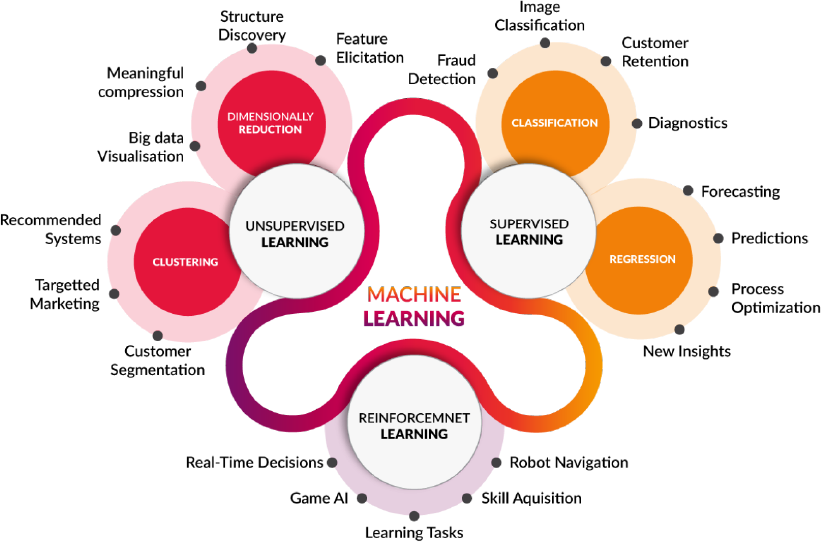
\includegraphics[width=\linewidth]{./img/machine_learning_sections.png}

\subsection{Natural Language Processing (NLP)}
\begin{itemize}
    \item Automated processing of human language (written \& spoken)
    \item Aims to understand and generate human (natural) language
    \item Understanding spoken text is still difficult
    \item Understanding written text became BIG business (search-engines)
    \item Generating human-like conversations is still very hard
\end{itemize}

\subsection{Dialogflow}
\textbf{Intents}
\begin{itemize}
    \item Recognizes the need of a user
    \item Require training to match to user inputs
    \item Follow up Intents (on Success)
    \item Fallback Intents (on Failure)
\end{itemize}
\textbf{Intent Matching (Recognize what your user want)}
\begin{itemize}
    \item For each intent, we provide examples for the various ways the user might communicate it
    \item Dialogflow uses this information to train a machine-learning model to understand not just the examples we've entered, but numerous other phrases that mean the same thing
\end{itemize}
\textbf{Entities/ Entity-Extraction}
\begin{itemize}
    \item Extract information from user inputs
    \item Help to identifiy required intent
    \item System Entities: (Date and time / Numbers / Amounts / Units / etc.)
    \item Developer Entities: defined by list of words (@pizza-type / @drink / etc.)
    \item User Entities: transient, temporary Information based on Conversation
\end{itemize}
\textbf{Dialog}
\begin{itemize}
    \item Linear: Gather a list of information
    \item Non Linear: Using Contexts
\end{itemize}
\textbf{Agents}
\begin{itemize}
    \item handles concurrent conversations with your end-users. It is a natural language understanding module that understands the nuances of human language. 
    \item is similar to a human call center agent
    \item top-level container for settings and data (intents, entities, knowledge, fullfillment..)
\end{itemize}
\textbf{Context}
\begin{itemize}
    \item Each Intent can have Input \& Output Context
    \item Intents are active based on active Context
    \item Expire automatically
\end{itemize}
\textbf{Fulfillment}
\begin{itemize}
    \item Action triggered on fullfilled Intents
    \item e.g. Webhook
\end{itemize}

\subsection{7 Steps of ML}
\begin{enumerate}
    \item Gathering data
    \item Preparing that data
    \item Choosing a model
    \item Training
    \item Evaluation
    \item Hyperparameter tuning
    \item Prediction
\end{enumerate}

\subsection{Algorithms}
\begin{itemize}
    \item \textit{Gradient Descent Algorithm}: linear regression, logistic regression, neural networks
    \item \textit{Distance-based Algorithm}: KNN, k-means
\end{itemize}